\chapter{Development of Cells with Metal End Windows}
\label{chap5}

\section{Overview}

Electron scattering experiments at JLab have traditionally used $^{3}$He targets made of glass due to the compatibility with spin-exchange optical pumping, the capability to be shaped into desired geometries through glass blowing, and the excellent nuclear spin relaxation properties. The borosilicate glass Pyrex had been the glass of choice prior to the discovery that the much less permeable aluminosilicate glass generally provides longer spin-relaxation time. The most recent targets were thus composed entirely of the aluminosilicate glass GE180.

After the 12 GeV upgrade, JLab plans to run experiments with much higher electron beam currents. The maximum current used before the upgrade was 15$\mu$A, while future experiments will be run at up to 60$\mu$A. We believe an all-glass target cell might survive long enough for an experiment with 30$\mu$A, but it is unlikely to survive at 60$\mu$A. A natural solution would be to replace the thin glass window (where electron beam enters and exits the target cell) with a material with higher strength and good spin-relaxation properties. 

Deninger~\emph{et al.}~\cite{Schmiedeskamp2006} from the Mainz group showed relaxation time of various metal surfaces: Mg (6 h), Al (6 h), Zn(12 h) etc. Gold caught our attention in particular, because it has a relatively long relaxation time of 20 h. This relaxation time was measured with the entire glass surface coated with gold, thus the area of gold surface was much larger than what will be needed for target windows. In addition, while the coating process made sure of the chemical purity, it did not make effort in ensuring the microscopic smoothness, which means the surface area was further increased. Therefore one would expect a even longer relaxation time with a smooth and smaller metallic surface. In light of this, our group have tested 19 cells with various geometries and materials, most of which incorporated a OFHC (oxygen-free high thermal conductivity) copper tube with gold coating. OFHC copper was chosen as the substrate in most cases because of its structural strengths and the familiarity with manufacturers. Towards the end of my work, we achieved a 15.6 h relaxation time with a Pyrex cell that had a 5'' long by 1'' gold coated copper tube attached horizontally. By extrapolating the relaxation rate due to gold surface from this result, we believe the relaxation rate introduced by small metal windows in a target cell will be less than 1/135 hr$^{-1}$. To the best of our knowledge, our group was the first to have proved the potential of incorporating metal to target cells in the presence of alkali vapor.

\section{Wall Relaxation of $^{3}$He}

\subsection{Relaxation on Glass Surfaces}

Fitzsimmons and Walters have studied surface-induced spin-lattice relaxation times as a function of temperature for $^{3}$He gas in glass containers~\cite{PhysRev.179.156}. There are mainly two categories of wall relaxation mechanisms: $^{3}$He adsorption on the glass surface and the permeation of $^{3}$He into glass. The latter mechanism can be greatly reduced by using impermeable aluminosilicate glass such as GE180. 

Timsit and Daniels~\cite{Timsit} then studied surface relaxation on a great number of common materials and presented a phenomenological model to describe the relaxation processes.For permeable glasses, the relaxation is determined by absorption of gas in the surface layer of the glass and by the paramagnetic impurity contents of the glass. The surface adsorption of $^{3}$He near paramagnetic sites on the walls also contributes to the nuclear relaxation. Relaxation due to absorption for permeable glasses will be discussed first below.

The diffusion coefficient $D$ of a noble gas in a glass can be calculated with the following equation:
\begin{equation}\label{D}
D=D_{0}e^{-Q_{d}/kT}
\end{equation}
where $Q_{d}$ is the activation energy for diffusion and $D_{0}$ is a constant. The diffusion coefficient can also be expressed with the mean diffusion jump distance of $^{3}$He atom in the glass $\langle\Delta r\rangle$ as:
\begin{equation}
D=\frac{\langle\Delta r\rangle^{2}}{6\tau}
\end{equation}
with $\tau$ being the mean time between diffusion jumps
\begin{equation}\label{residence_time}
\tau=\tau_{0}e^{E_{dif}/kT}
\end{equation}
where $\tau_{0}=\langle\Delta r\rangle^{2}/6D_{0}$.

Let $n_{g}$ be the number of atoms dissolved in the surface layer of mean thickness $\langle\Delta r\rangle$, the rate at which $^{3}$He atoms enter and leave the surface layer of the glass is then $n_{g}/6\tau$~\cite{Timsit}. $n_{g}$ should be proportional to the solubility $S$ of $^{3}$He in the glass, so for a spherical cell
\begin{equation}\label{absorption_ng}
n_{g}=\frac{6NkT\langle\Delta r\rangle S}{d}
\end{equation}
where d is the diameter of the cell, N is the total number of free $^{3}$He atoms.

For most trapping sites in the glass, the intrinsic relaxation time $T_{i}$ is longer than $\tau$ which is the time it takes for $^{3}$He to leave the $\langle\Delta r\rangle$ layer. However, $T_{i}$ for a paramagnetic site is shorter than $\tau$, thus will completely relax the nuclear spin of a $^{3}$He atom. The relaxation time of $^{3}$He in permeable glass cells is controlled by absorption of the atoms in the surface layer at paramagnetic sites. The average nuclear relaxation time of a $^{3}$He trapped in the glass close to a Fe$^{3+}$ ion (one common type of paramagnetic impurity in glass) is~\cite{Abragam}:
\begin{equation}
\frac{1}{T_i}\approx\frac{3}{5}\frac{\mu_{He}^{2}\mu_{B}^{2}g^2}
{\hbar^2b^6}\frac{T_{Fe}}{1+\omega_0^2T_{Fe}^2}
\end{equation}
where $\mu_{He}$ is the nuclear dipole moment of $^{3}$He, $\mu_B$ is the Bohr magneton, g is the g factor of the Fe$^{3+}$ ($^{6}S_{5/2}$) ion, and b is the distance between the spins. Taking b as 1 $\mathring{A}$ and g as 5.9~\cite{Kittel}, $T_i$ is $\sim10^{-11}$ s, which is 10 times smaller than the shortest $\tau$.

Even a small amount of paramagnetic impurities among the trapping sites in the glass can provide dominating contribution on the $^{3}$He spin relaxation. Assuming during the random walk of $^{3}$He atom in the glass, there are on average $\beta$ atoms in its vicinity, and atom fraction of paramagnetic impurities is $N_{impurity}$, the relaxation time due to absorption is if $T_i\ll\tau$:
\begin{equation}\label{T_ab}
T_{ab}=\frac{6N\tau}{\beta N_{impurity}n_g}
\end{equation}

For impermeable glasses such as GE180, the relaxation rate due to absorption into the glass walls is typically negligible. The dominating relaxation mechanism here is adsorption of $^{3}$He on the glass wall in vicinity of a paramagnetic site.

The sticking time $\tau_s$ is given by Frenkel's Law~\cite{Frenkel}:
\begin{equation}\label{sticking_time}
\tau_s=\tau_{s0}e^{E_{ad}/kT}
\end{equation}
where $\tau_{s0}$ is on the order of $10^{-13}$ s for most solid surfaces~\cite{Frenkel}, $E_{ad}$ is the adsorption energy. At room temperature, we have $\tau_s\sim\tau_{s0}\sim 10^{-13}$ s. The number of atoms hitting the wall per unit time and unit area is given by $\frac{1}{4}n\bar{v}$, where n is the number density of $^{3}$He gas and $\bar{v}$ is the mean velocity. For a spherical cell with diameter d, the number of atoms adsorbed on the wall is
\begin{equation}\label{adsorption_ng}
n_{g}'=\frac{3N\bar{v}\tau_s}{2d}
\end{equation}

The intrinsic relaxation time $T_i'$ of a $^{3}$He near a paramagnetic site on the wall is much longer than the sticking time $\tau_s$. The average number of collisions required to depolarize $^{3}$He is $T_i'/\tau_s$, thus the relaxation time due to adsorption is
\begin{equation}\label{T_ad}
T_{ad}=\frac{NT_i'}{N_{impurity}n_g'}
\end{equation}

The total relaxation rate is the sum of that due to adsorption and absorption (for permeable glasses):
\begin{equation}
\frac{1}{T_{wall}}=\frac{1}{T_{ad}}+\frac{1}{T_{ab}}
\end{equation}

Substitute Eq.~\ref{residence_time},~\ref{absorption_ng} into Eq.~\ref{T_ab} and Eq.~\ref{sticking_time},~\ref{adsorption_ng} into Eq.~\ref{T_ad}, the wall relaxation rate can be written as
\begin{equation}
\begin{split}
\frac{1}{T_{wall}}=&\frac{\beta N_{impurity}kT\langle\Delta r\rangle S}{d\tau_0}e^{-E_{dif}/kT}\\
&+\frac{3N_{impurity}\bar{v}\tau_{s0}}{2dT_i'}e^{E_{ad}/kT}
\end{split}
\end{equation}

According to the above equation, both the diffusion-induced and the surface-induced relaxation rates are proportional to the surface-volume ratio of the cell, \emph{i.e.} to the inverse of the cell diameter $d$. Thus it is useful to describe the surface relaxation properties with a physical quantity $\rho$, which is commonly referred to as the "relaxivity". The relaxivity is independent of cell geometry and is related to the wall relaxation rate $1/T_{wall}$, the surface to volume ratio $A/V$ by the following equation:
\begin{equation}
1/T_{wall}=\rho A/V
\end{equation}

Fitzsimmons~\emph{et al.}~\cite{PhysRev.179.156} found by using impermeable aluminosilicate glass, the relaxation due to absorption can be greatly reduced thus increasing the total relaxation time. Heil~\emph{et al.} reported~\cite{PhysRevA.201.337} glass cells that were internally coated with metallic films provided even longer relaxation time. Ce was one of the metals that greatly reduced wall relaxation rate as it blocks $^{3}$He atoms from diffusing into the glass walls and it also has a low adsorption energy which leads to very short sticking time. For SEOP (Spin-Exchange Optical Pumping), we automatically profit from the Rb film which covers the inner surface of the pumping chamber. Similarly, another way to eliminate relaxation due to absorption is to coat the inner surface with sol-gel~\cite{solgel}. It is a mixture of aluminum nitrate nonahydrate $Al(NO_3)_39H_2O$, ethanol and deionized water. The sol-gel coating also improves relaxation time by blocking $^{3}$He atoms from diffusing into the glass.

\subsection{Relaxation on Metal Surfaces}

Since $^{3}$He gas does not diffuse into metals~\cite{barrer}, the relaxation is purely due to surface effects. However, the surface-induced relaxation on metal surfaces is not yet well understood. There are two additional relaxation mechanisms with metal surfaces compared to those for glass. First mechanism is the depolarization of $^{3}$He nuclei near the metal surface by oscillating magnetic field from eddy currents induced by the movement of these same nuclear dipoles. Smythe~\cite{Smythe} derived the magnetic field generated by eddy current induced in a metal sheet by a moving magnetic dipole using the method of images. Timsit~\emph{et al.}~\cite{Timsit} estimated the relaxation due to eddy currents using the same method:
\begin{equation}
\frac{1}{T_m} = \frac{3\times 10^{-4}}{\pi} \frac{\mu_{He}^4}{\bar{v}r_{0}^{4}\hbar^{2}}\frac{A_p}{d^3}
\end{equation}
where $\bar{v}$ is the mean velocity of atoms, $r_0$ is the closest distance of the nucleus to the metal surface, d is the cell diameter, $A_p$ is the area. According to Timsit~\emph{et al.}~\cite{Timsit}, $T_m$ is on the order of $10^{16}$ s if $r_0=1\mathring{A}$ and $A_p = 9.2cm^2$. Even though the area of the cell is usually much larger in our study and other parameters may take different values, but it should still remain true that the relaxation rate of $^{3}$He due to eddy currents can by safely neglected.

The second additional mechanism that contributes for relaxation of $^{3}$He adsorbed on the metal surfaces is the Korringa scattering. Nuclear spin relaxes when the nucleus interacts with conduction electrons in the metal, where the an electron flips its spin and the spin state of the nucleus changes. The Pauli exclusion principle states that the interaction is only allowed when the final state the electron jumps to is initially unoccupied. Thus according to Fermi statistics, only electrons with energy close (approximately within kT) to the Fermi energy level can participate in such interactions. Slichter~\cite{Slichter} has derived the Korringa relaxation rate in metal to be:
\begin{equation}
\frac{1}{T_K}=\frac{(4\pi)^6}{9h^7}(g_s\mu_B \frac{\mu_K}{K})^2 \eta^4m^3\epsilon_F kT
\end{equation}

To calculate the total Korringa relaxation rate due to metal surface, one needs to consider the overlapping of wave functions of the conduction electrons and the nuclei of adsorbed $^{3}$He atoms in the vicinity of the metal surface. Nelson~\cite{NelsonThesis} derived the total surface Korringa relaxation as:
\begin{equation}
\frac{1}{T}=\frac{1}{T_K}\frac{S}{V}\int_{0}^{\infty} f\left(l\right)^2 e^{-U\left(l\right)/kT}dl
\end{equation}
where S and V are the surface area of the metal and total volume of the cell, respectively, $U\left(l\right)$ is the atom-surface potential with the edge of the metal taken as $l=0$, $f\left(l\right)$ is the fractional density of conduction electrons outside the surface. Nelson further used the work function of the metal to estimate $f\left(l\right)$, and assumed a van der Waals form for $U\left(l\right)$. His calculations suggest that the Korringa relaxation times for $^{3}$He on various metal surfaces should be thousands of years, including the metal of interest for our studies, gold.

If eddy currents and Korringa relaxation are the only surface relaxation mechanisms, we would have very long lifetime for our test metal cells. Unfortunately, our series of studies have shown relaxation times to be between a few hours and 16 hours most of the time, for which both aforementioned relaxation mechanisms can be safely neglected. Although the dominating relaxation mechanism is still not well understood and significantly faster than those we have better understanding about, the results of our studies are still promising, as they suggest the extra relaxation rate due to use of metal end windows should still be small enough and allow future experiments to run at 60$\mu$A electron beam current.

\section{Test Cell Fabrication}

\subsection{Overview}

In order to study the relaxation rate due to metal surface, we have created and tested 19 cells so far, most of which contained metal tubes. The metal tubes are 5'' in length and have 1'' outer diameter, 3'' of glass tubes are attached to both ends via Houskeeper seal. The total area of the metal surface is 101.3 $cm^2$, and is far larger than what will be for metal end windows. This large geometry is chosen to intentionally increase the relaxation rate for studying. This particular design of metal tube is also favored for the convenience of manufacturing, as we were expecting a large number of test cells to be studied and any design that could save time would potentially lead to a much shorter test time before finding the final design.

The making of these test cells usually includes five steps (except control cells with pure glass and cells without gold coating):

1. Larson Electronic Glass~\cite{Larson} provides us a glass--metal--glass tube that uses Houskeeper seal to bond glass and metal together.

2. The machine shop in the physics department of University of Virginia then mechanically polishes the inside of the metal tube.

3. Able\cite{Able} Electropolishing electropolishes the metal tube.

4. Epner\cite{Epner} Technology Inc. electroplates the metal tube with gold.

5. Mike Souza at Princeton University, our glass blower, resizes the glass from stock material and makes the final cell with our desired dimensions and attaches the metal tube to the glass cell. The resizing is for removing micro-fissures from the glass surface and reducing wall relaxation rates~\cite{Cates1993}.

Each step will be described below.

\subsection{Glass-Metal Seal}

Larson Electronic Glass made the glass-metal-glass tubes for us, Fig.~\ref{metal_tube} is a picture of one of the tubes used in our tests. The glass-metal seal used by Larson is known as the Houskeeper seal~\cite{Houskeeper}. The outside of the copper tube is machined down to a knife edge and is wetted with glass. The edge of copper is usually heated before covering with glass. The heating process creates a thin layer of crimson-color copper oxide as can be seen in Fig.~\ref{metal_tube}. Houskeeper seals were originally used for vacuum, we checked each seal down to the $10^{-10}mbar\cdot l/s$ level. To make sure these seals will survive the high pressure JLab experiments, we also tested the integrity of them under up to 20 atm for extended period of time.

\begin{figure}[t!]
	\centering
	\resizebox{0.91\textwidth}{!}{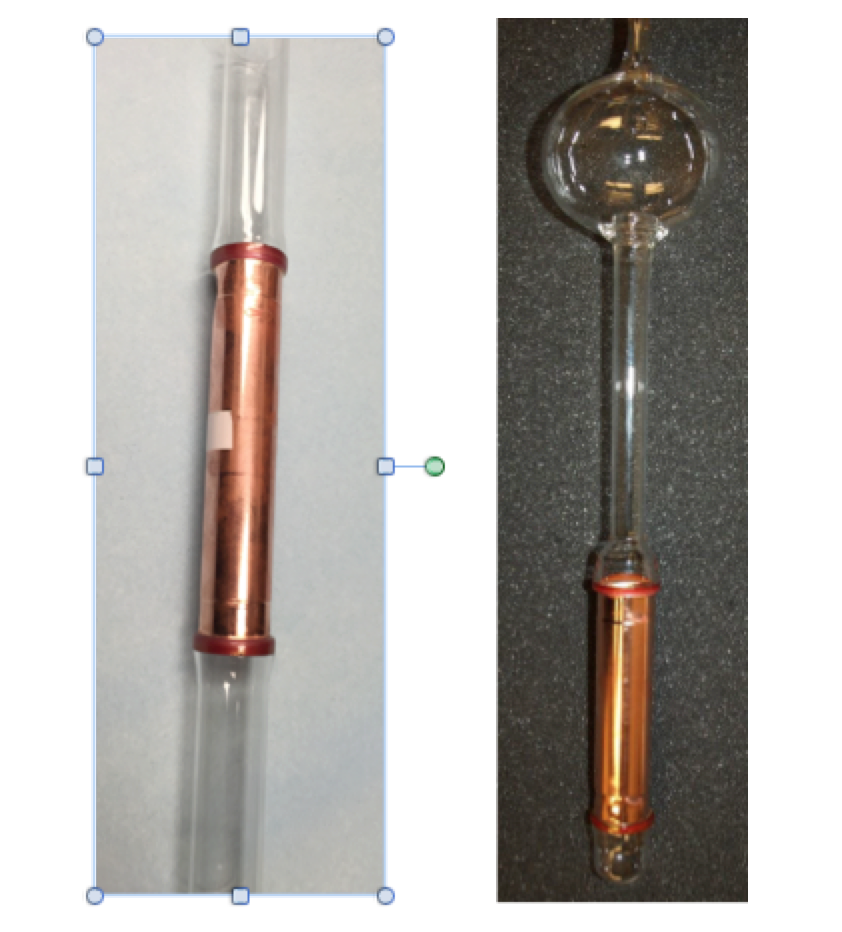
\includegraphics{metal_tube.png}}
	\caption{{Shown is a glass--metal--glass seal. The metal tube is 5'' long by 1'' outer diameter. The glass is wetted onto the knife-edge of copper on both ends.}}
	\label{metal_tube}
\end{figure}

\begin{figure}[t!]
	\centering
	\resizebox{0.91\textwidth}{!}{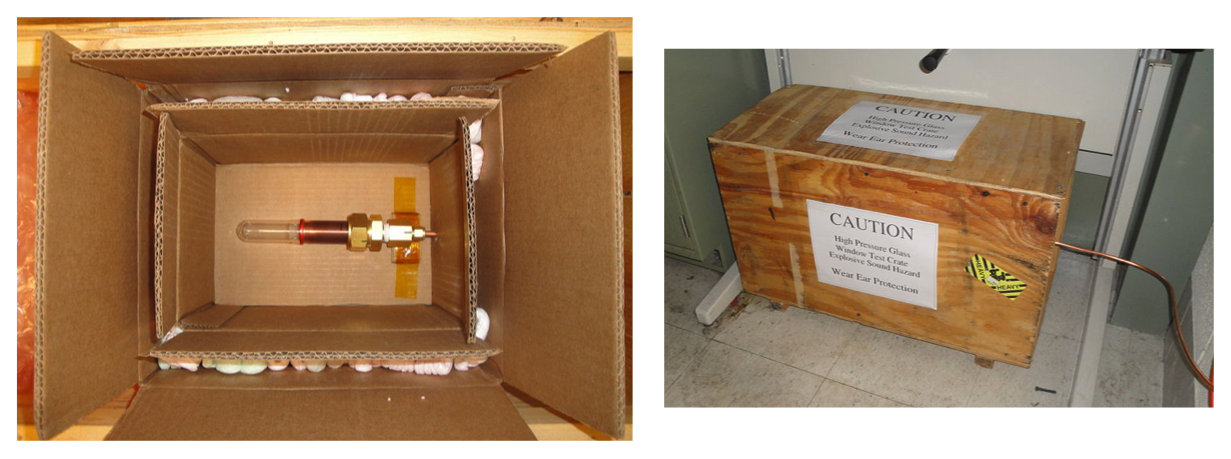
\includegraphics{pressure_test.png}}
	\caption{{Glass-metal seals survived pressure higher than 20 atm.}}
	\label{pressure_test}
\end{figure}

The copper used in our tests is OFHC (oxygen-free high thermal conductivity) copper. In the earlier stage of our tests, OFHC copper was attached to the Pyrex glass, in which case a direct connection could be made. For the later tests where we were moving closer to the final goal of using metal end windows with the impermeable aluminosilicate glass GE180, a transition glass between OFHC copper and GE180 had to be used. The coefficient of expansion for GE180 glass is not compatible for making a direct seal with OFHC copper, thus Corning 7052 Kovar sealing glass was used as the transition. The two materials connected by a seal should have similar coefficients of expansion, the 7052 Kovar sealing glass serves as an intermediate material to bridge the gap between OFHC copper and GE180. The other type of metal used in our glass--metal seals was titanium, for which only Pyrex was used.

\subsection{Mechanical Polishing and Electropolishing}

The mechanical polishing is done by our machine shop in the department. A wire brush attached to a lathe was placed inside the tube while the lathe spun. This first-step polishing produced a relatively smooth surface in preparation for the following electropolishing process.

After the tubes were mechanically polished by the machine shop, they were sent to Able for electropolishing. The tube serves as the cathode, whihc is immersed in a temperature-controlled bath of electrolyte and connected to the positive terminal of a DC power supply, while the cathode is the attached to the negative terminal. During electropolishing, the polarized film is subjected to combined effects of gassing (oxygen) that occurs with electrochemical metal removal, saturation of the surface with dissolved metal and the agitation and temperature of the electrolyte. Metal on the surface is oxidized and dissolved in the electrolyte, the microscopic high points on the surface dissolve faster than the rate of attack on the other parts of the surface, which provides a smoothing effect. As a result, the electropolishing process removes a thin layer of metal (about 20 $\mu m$ for our tubes), leaving a microscopically smooth and featureless surface. By contrast, even a fine mechanically polished surface will still show smears and other directionally oriented patterns or effects\cite{Electropolishing}. Fig.~\ref{Electropolishing} shows a diagram of the polishing process and its smoothing effect.

\begin{figure}[t!]
	\centering
	\resizebox{0.91\textwidth}{!}{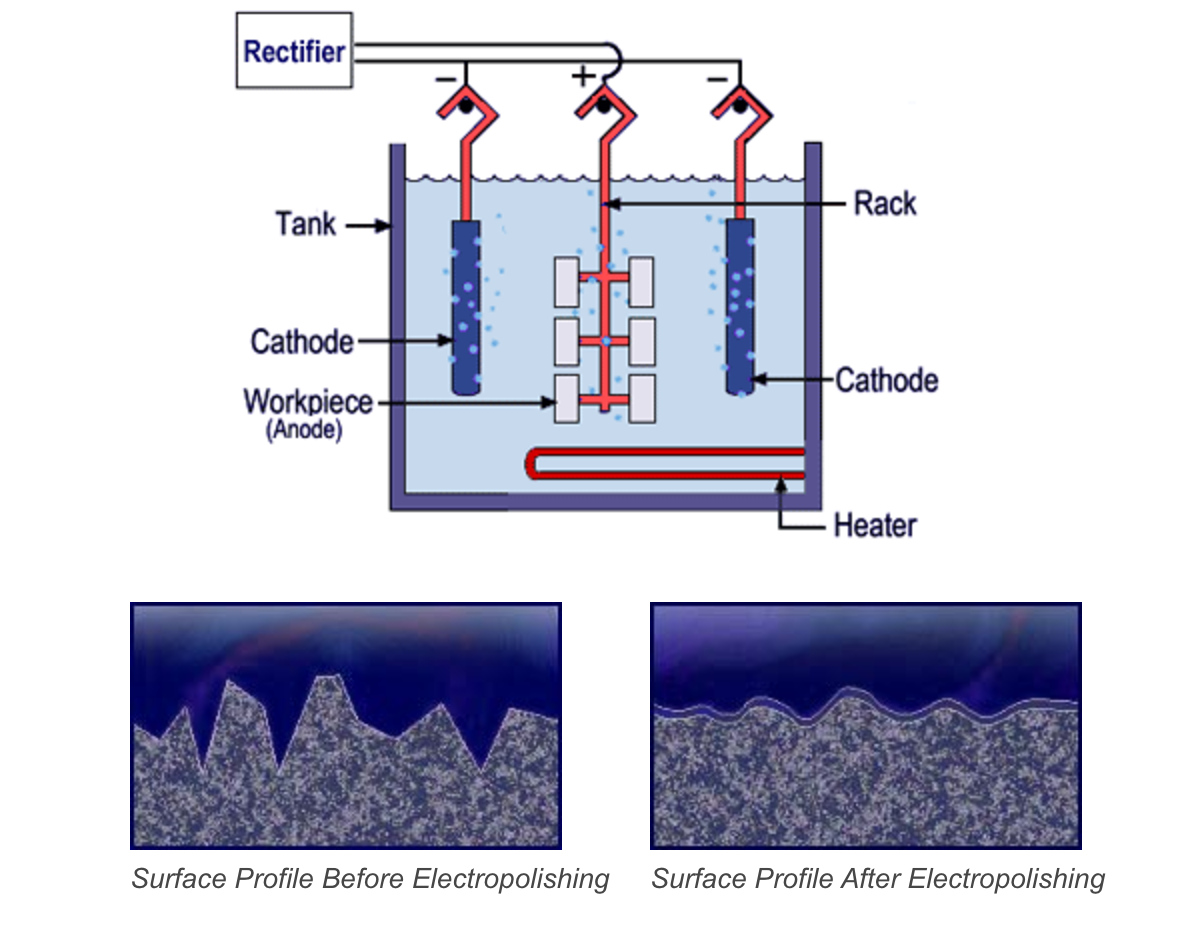
\includegraphics{Electropolishing.png}}
	\caption{{Electropolishing~\cite{Electropolishing}}}
	\label{Electropolishing}
\end{figure}

\subsection{Electroplating}

As stated earlier, because of the good lifetime reported by Deninger~\emph{et al.}\cite{Deninger2006}, gold was plated on the inner surface of the OFHC copper and titanium tubes. Epner Technology Inc. handled the electroplating for us. Electroplating is the reverse process of electropolishing. When electric current passes through the electrolyte, the electrolyte splits up and some of the desired metal atoms it contains are deposited in a thin layer on top of the electrodes. Nickel and chromium are two common undercoatings used for electroplating, however, they are both ferromagnetic and cannot be used for us as they would introduce additional spin relaxations. As a result, Epner used a copper strike to improve the durability of gold coating. A 5 $\mu m$ layer of gold was subsequently electroplated on the inner surface of the tubes. Fig.\ref{gold_coating} shows a comparison of a OFHC copper tube with gold-coating and a tube without any coating. 

\begin{figure}[t!]
	\centering
	\resizebox{0.91\textwidth}{!}{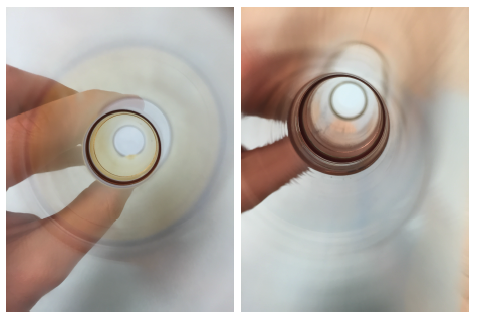
\includegraphics{gold_coating.png}}
	\caption{{Shown left is the inner surface of a gold coated OFHC copper tube. Shown right is a OFHC copper tube without coating.}}
	\label{gold_coating}
\end{figure}

\subsection{Final Assembly of the Cell}

After the tubes were coated, shipped back to us and leak checked one more time, they were cleaned with our ultrasonic cleaner. Fig.~\ref{ultrasonic_cleaner} shows the setup of the cleaning process. We cleaned the impurities on the surfaces of the tubes with ethanol, deionized water and methanol for thirty minutes each. As shown in the figure, a beaker containing the chemical solution and the tubes were placed in water bath inside the ultrasonic cleaner. Because of the dimensions of the cleaner and the beaker, we cleaned one end of the tubes first then flipped them to clean the other end before switching solution.

\begin{figure}[H]
	\centering
	\resizebox{0.4\textwidth}{!}{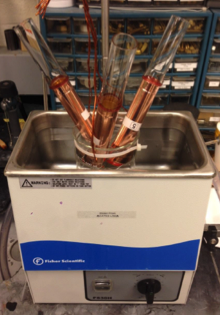
\includegraphics{ultrasonic_cleaner.png}}
	\caption{{Ultrasonic cleaner with 3 tubes being cleaned.}}
	\label{ultrasonic_cleaner}
\end{figure}

The test tubes were then shipped to our glassblower Mike Souza at Princeton University. All glass was reblown to the right size to reduce micro-fissures which would lead to high relaxation rate. The test tube was spliced to transfer tube and pumping chamber. A string (see Fig.~\ref{string}) which would be used for cell filling was also made at Pricenton. Traditionally, a pure glass cell would be placed entirely in a oven for annealing. A cell made with GE180 would go through a five-minute ramping time to 780$^{\circ}C$, stay at 780$^{\circ}C$ for five minutes and slowly cool down to room temperature for at least 5 hours~\cite{DanThesis}. A Pyrex cell would be annealed in the exact same way except the highest temperature is 565$^{\circ}C$. However, most our test cells could not have been annealed in the same way because of the glass-metal seal. Had we expose the seal to high temperature for long period of time, gold atoms might have migrated into the metal substrate and the seal might even break. Thus the metal tubes were attached to the rest of the glass parts after the pure glass parts were annealed. 

\begin{figure}[t!]
	\centering
	\resizebox{0.91\textwidth}{!}{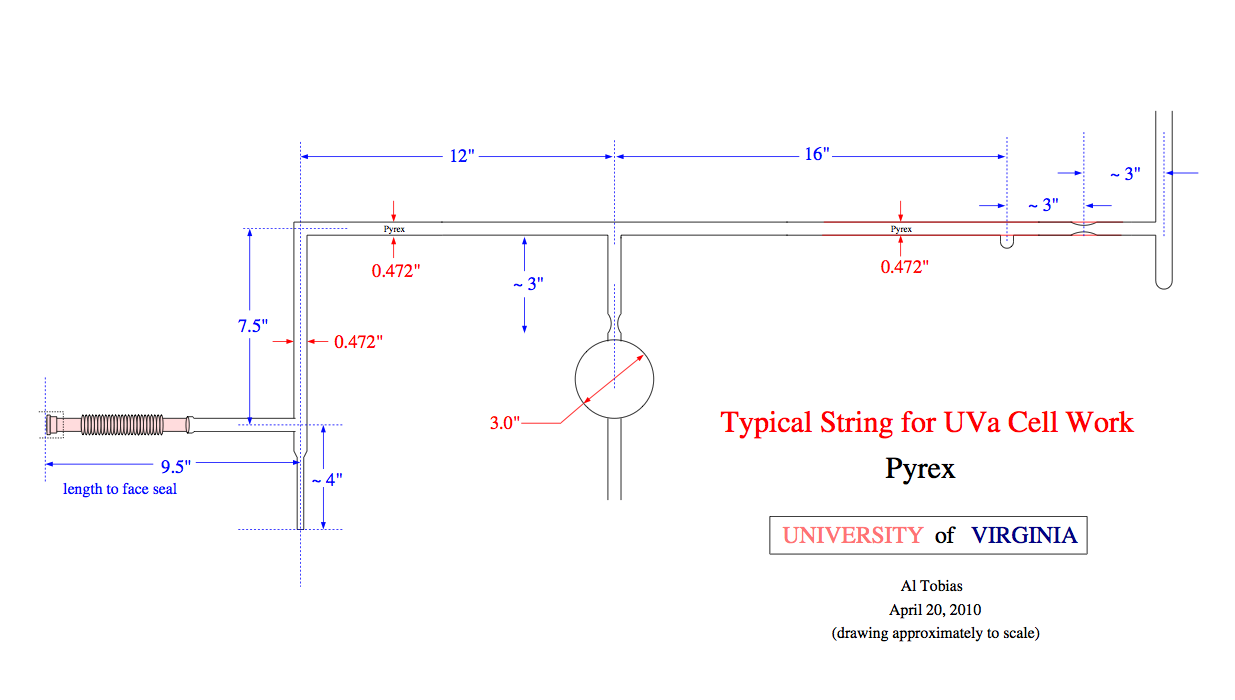
\includegraphics{string.png}}
	\caption{{Shown is the design of a typical string for our test cells.}}
	\label{string}
\end{figure}

\section{Cell Fill Procedure}

The details of cell fill was described thoroughly by Matyas~\cite{DanThesis}, I will briefly cover the process for the sake of completeness.

\subsection{Cell Fill Preparation}

Although the actual cell fill work only took less than a day, the preparation that led to the fill usually took 10-15 days. The string, cell and the retort were spliced together and attached to our homemade gas system through the bellows. a pre-scored ampoule of alkali metal was dropped from the top the of the retort.  Fig.~\ref{cell_gas_system} is a diagram of the string, cell and retort all connected together. 

\begin{figure}[t!]
	\centering
	\resizebox{0.91\textwidth}{!}{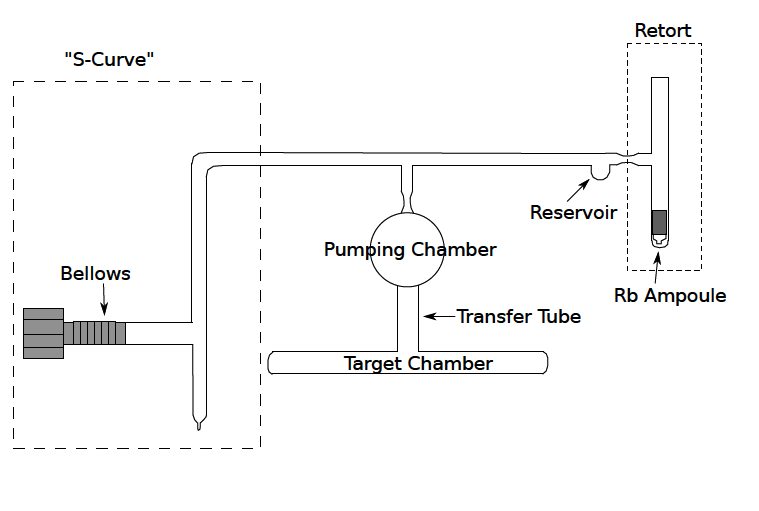
\includegraphics{cell_gas_system.png}}
	\caption{{A diagram of a Pyrex string with a cell and a retort attached while connected to the gas system through the bellows. Adapted from Matyas~\cite{DanThesis}.}}
	\label{cell_gas_system}
\end{figure}

The entire system was first rough-pumped down with a mechanical pump, and then kept being pumped by a diffusion pump to even higher vacuum. After the system was pumped for a few days and alkali metal was added in the system, we would keep pumping the system with the diffusion pump for roughly a week. To prevent the hot oil in the diffusion pump from going up into the gas system and the cell, a cold trap above the diffusion pump was filled every day with liquid nitrogen. "Flamebakes" were also performed 2-3 times each day during the one-week pumping period. A methane-oxygen torch was used to gently bake on the glass in the flamebakes. The bake should start from the retort which is the farthest away from the diffusion pump, and move slowly towards the bellows, so the impurities chased off the inner surfaces can be ``swept" towards the pump leaving as few impurities behind as possible. The alkali metal was typically melted in the retort on the second or third flamebake and should be melted during each of the remaining flamebakes. On the day before the fill, alkali metal was melted and chased into the pumping chamber.

\subsection{Cell Fill}

The first thing on the fill day was to pump all portions of the gas system to vacuum and selectively back fill some parts with appropriate gases (either N$_2$ or $^{3}$He) to minimize outgassing. The gas filled into the cell should always be cleaned during the path to the cell. Earlier test cells were filled with the noble gas purifier while the later cells were done with a homemade cryogenic trap.

The homemade cryogenic trap consisted of a copper tubing placed inside a box-shaped Dewar. The Dewar was filled with liquid nitrogen when filling N$_2$ and liquid helium when filling $^{3}$He, so impurities in the gas were frozen in the copper tubing. Temperature inside the dewar was monitored with two silicon diodes to determine whether copper tubing was fully submerged in the cold liquid.

The volume of the cell was also determined during the fill process. A Baratron pressure gauge was used to measure a calibrated volume (CV) of 992.9 cc. 300 Torr of gas was filled into the calibrated volume, then the valve on CV was closed and any gas outside of CV was pumped away. Next the gas kept in CV was let out into the fill gap between CV and the string, then into the cell while monitoring pressure with the Baratron gauge, thus the volume of the cell could be calculated with ideal gas law.

Around 70 Torr of nitrogen was put into the cell before filling $^{3}$He. To prevent nitrogen from escaping the cell while filling $^{3}$He, the string valve was kept closed until $^{3}$He pressure in fill gap rose well above 70 Torr. A total gas pressure of just under 760 Torr (1 atm) was reached. This target pressure was chosen because when the connection between the cell and the string was melted, the atmospheric pressure would collapse it and seal the cell for us. All cells except Kappa1 contained pure rubidium, while Kappa1 contained 5:1 alkali mixture of potassium to rubidium.

\section{Experimental Setup and Procedure}

All cells incorporated metal were tested with Pulse NMR as it only affects a small region of the cell and minimizes influences from eddy current in the metal tubes. Kappa1 was a simple spheric and pure GE180 cell, which was built to rule out the possibility that the melt of GE180 our cells had been made of was bad. Because of its lack of metal and lack of convenient places to wrap pickup coils on, Adiabatic Fast Passage was used to test Kappa1. Both PNMR and AFP were discussed in a general way in chapter 3, I will only add to the discussions with more specific experimental setups for this study. Spindown measurements were the main means of studying relaxation properties, I will also discuss how we used spindowns with different sampling rate to extract PNMR losses and lifetime corrected for such losses.

\subsection{Pickup Coils}

In a AFP measurement, pickup coils are placed next to the side windows of the oven. However, the same setup proved to be more difficult for us to receive high-quality PNMR signals. To keep the pickup coils from the heat of the oven, we manually wrap a solenoid coil on the transfer tube of test cells where it is approximately 2'' below the bottom of the oven. These coils were made with 40-50 turns of AWG 20 copper wire. Because of the off-center positions of the pickup coils, inhomogeneities were significant enough to affect FID signals, gradient coils were used to cancel such inhomogeneities.

\subsection{Gradient Coils}

Inhomogeneities were canceled to the best we could empirically with three sets of gradient coils. Each set of gradients coils consists of two oppositely wound coils separated by a distance $d$, this particular type of coils are referred to as "Maxwell coils". The setup is very similar to that of Helmholtz coils, except the opposite direction of currents and the larger optimum separation $d=\sqrt{3}R$, where $R$ is the radius of the coils. The opposite direction is to cancel out the magnetic field at the center, and the optimum separation makes the first four leading terms in the Taylor expansion of the inhomogeneities zero\cite{Callaghan}. Fig.\ref{gradient_coils} shows the coil orientations. The z axis is defined to be aligned with the direction of the holding field while x and y axes are in the transverse plane. The direction of coil axis is then defined by the angle $\theta$ and $\phi$, where $\theta$ is with respect to the z axis and $\phi$ is the azimuthal angle in the x-y plane.

\begin{figure}[t!]
	\centering
	\resizebox{0.91\textwidth}{!}{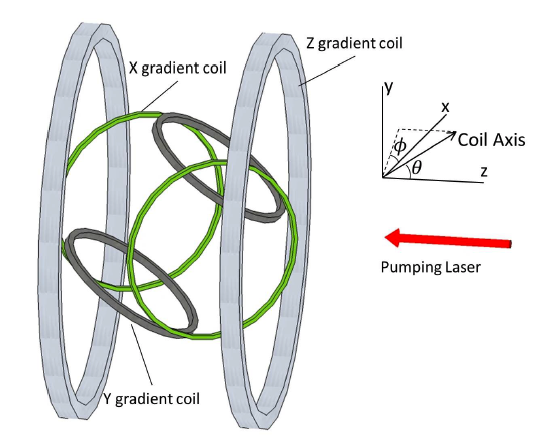
\includegraphics{gradient_coils.png}}
	\caption{{Diagram of the coils. Adapted from Zheng~\cite{YuanThesis}.}}
	\label{gradient_coils}
\end{figure}

The magnetic field at the center is given by\cite{PhysRevA.37.2877}

\begin{equation}\label{gradient}
\begin{split}
\nabla\boldsymbol{B}(\theta, \phi)
&=\begin{bmatrix}
\partial B_x/\partial x & \partial B_y/\partial x & \partial B_z/\partial x \\
\partial B_x/\partial y & \partial B_y/\partial y & \partial B_z/\partial y \\
\partial B_x/\partial z & \partial B_y/\partial z & \partial B_z/\partial z
\end{bmatrix}\\
&=3\kappa I
\begin{bmatrix}
sin^2\theta cos^2\phi-\frac{1}{3} & sin^2\theta sin\phi cos\phi & sin\theta cos\theta cos\phi \\
sin^2\theta sin\phi cos\phi & sin^2\theta sin^2\phi-\frac{1}{3} & sin\theta cos\theta sin\phi \\
sin\theta cos\theta cos\phi & sin\theta cos\theta sin\phi & cos^2\theta-\frac{1}{3}
\end{bmatrix}
\end{split}
\end{equation}
where the calibration constant $\kappa$ is:

\begin{equation}
\kappa = \frac{3\pi n R^2 d/2}{5(d^2/4+R^2)^{5/2}}G\,cm\,A^{-1}
\end{equation}

The most important terms in Eq.\ref{gradient} are those related to $B_z$: $\partial B_z/\partial x$, $\partial B_z/\partial y$ and $\partial B_z/\partial z$. The orientations of the gradient coils can be chosen such that each of the three sets of coils controls one of the aforementioned terms. This "magic angle" $\theta_m$ is given by

\begin{equation}
\theta_m = cos^{-1}1/\sqrt{3}=54.7^{\circ}
\end{equation}

For $\theta=\theta_m$ and $\phi=0$ the gradient tensor is

\begin{equation}
\nabla\boldsymbol{B}(\theta_m, 0)=\kappa I
\begin{bmatrix}
1 & 0 & \sqrt{2}\\
0 & -1 & 0 \\
\sqrt{2} & 0 & 0
\end{bmatrix}
\end{equation}

For $\theta=\theta_m$ and $\phi=\pi/2$ we have

\begin{equation}
\nabla\boldsymbol{B}(\theta_m, 0)=\kappa I
\begin{bmatrix}
-1 & 0 & 0\\
0 & 1 & \sqrt{2}\\
0 & \sqrt{2} & 0
\end{bmatrix}
\end{equation}

Finally, for the z gradient coil we have

\begin{equation}
\nabla\boldsymbol{B}(\theta_m, 0)=\kappa I
\begin{bmatrix}
-1 & 0 & 0\\
0 & -1 & 0\\
0 & 0 & 2
\end{bmatrix}
\end{equation}

Our gradient coils were built by Zheng~\cite{YuanThesis}. The separations do not follow the optimum condition $d=\sqrt{3}R$ due to spatial limitations. The dimensions of the gradient coils are shown in Table~\ref{gradient_coils_table}.

\begin{center}
	\begin{tabular}{ | c | c| c| c | }
		\hline
		& turns & radius & separation \\ \hline
		x & 42 & 33 cm & 64 cm \\ \hline 
		y & 100 & 28 cm & 56 cm \\ \hline
		z & 8 & 66 cm & 66 cm \\
		\hline
	\end{tabular}
\end{center}\label{gradient_coils_table}

\subsection{Laser Setup}

In earlier stage of the study, narrow-band Commet laser from Newport was used. Each Commet laser provides roughly 20 W power, the optical fibers were combined through a combiner which requires water cooling if multiple lasers are used at the same time. In later studies, single Raytum laser was used instead as it can provide much higher power. Both Commet laser and Raytum laser have around 0.2 nm FWHM (full width at half maximum).

Fig.~\ref{optics} shows a diagram of the optics used for SEOP (spin-exchange optical pumping). After the combiner, laser was focused by two lenses L1 and L2 such that the power spread enough to not damage the polarizing cube and was focused to an appropriate size at the cell position. The polarizing cube separated the beam into two beams with orthogonal linear polarizations. The beam with polarization parallel to this plane went through the cube, and the other beam with polarization perpendicular to the plane was reflected. The reflected beam went through a QWP (quarter wave plate), reflected at a mirror, went through the QWP one more time. Its polarization was changed to be parallel to this plane at this point and went through the cube. This beam is referred to as the "main beam" as it is ideally aligned with the holding field. The beam that went through the cube the first time was sent towards the oven by a mirror. Because of the small angle relative to the main beam, this is called the "skew beam". Both the main beam and the skew beam went through QWP before arriving at the oven window and were turned to circular polarization in the same direction.

\begin{figure}[t!]
	\centering
	\resizebox{0.91\textwidth}{!}{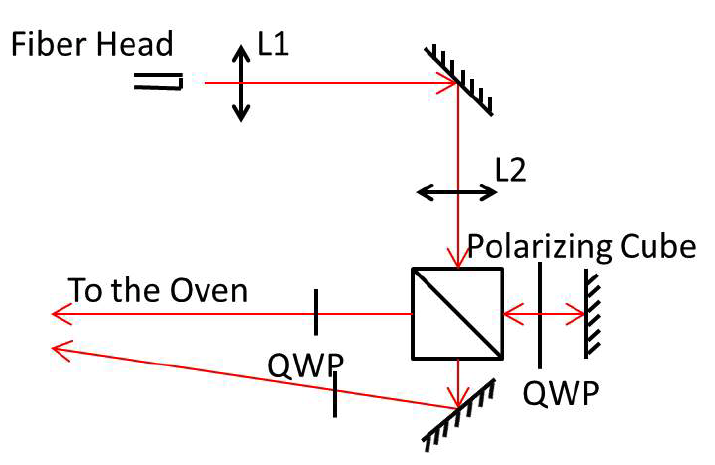
\includegraphics{optics.png}}
	\caption{{Optics for spin-exchange optical pumping. Adopted from Zheng~\cite{YuanThesis}.}}
	\label{optics}
\end{figure}

\subsection{PNMR Losses and Corrected Lifetime}

As described in chapter 3, there are generally two methods for us to determine polarization losses due to measurements: one is to take several measurements quickly enough that all depolarization can be attributed to measurement losses, the second method is to take multiple spindown measurements each with a different sampling rate. PNMR measurements cause a fraction of longitudinal polarization to be lost, two adjacent measurements require a long enough separation so the depolarization effect can be fully dispersed. For this reason, the first method mentioned above is not an option for PNMR. We have applied the second method to most of the 19 test cells that had lifetime of at least a few hours.

A spindown is typically a series of measurements of FID (Free Induction Decay) signals. Obtaining a good FID signal generally requires tuning the holding magnetic field and the gradient settings to reduce inhomogeneities.

\begin{figure}[t!]
	\centering
	\resizebox{0.91\textwidth}{!}{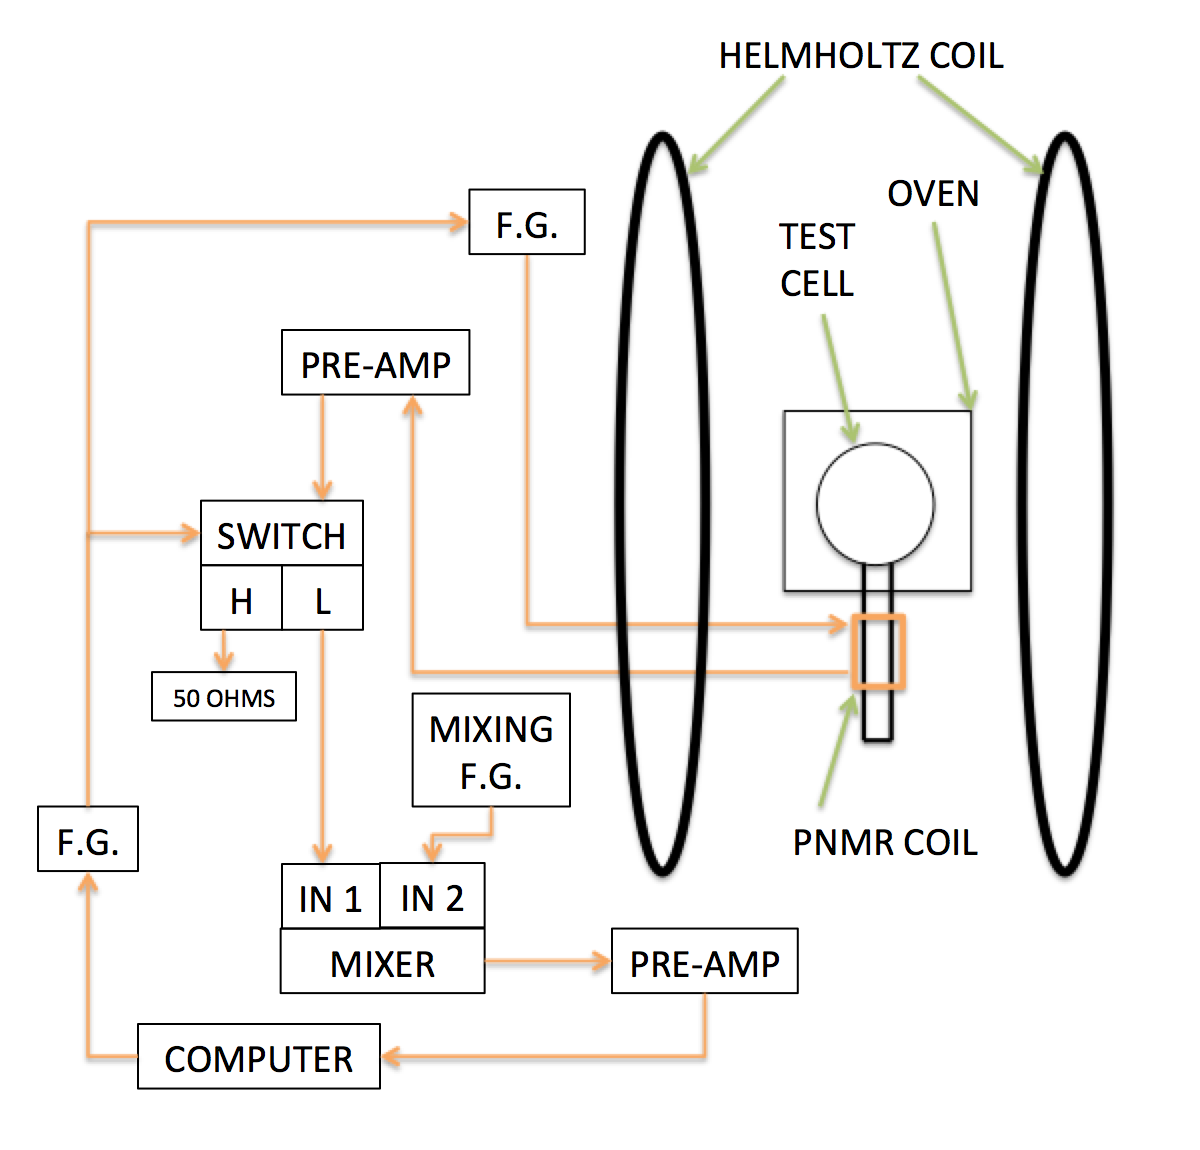
\includegraphics{PNMR_setup.png}}
	\caption{{\bf PNMR setup.}}
	\label{PNMR_setup}
\end{figure}

In a PNMR measurement, it is important that the RF frequency is the correct Larmor frequency of the holding field. The RF frequency was set to be at 56.6 kHz, it was often the case the holding field would start being off-resonance at the beginning.  As Fig.~\ref{PNMR_setup} shows, the final recorded signal was the absolute value of the difference between the signal frequency and the mixing frequency, which does not provide information about whether the frequency of the signal (which was proportional to the holding field) was above (or below) the mixing frequency. By intentionally changing the mixing frequency by an appropriate amount, we were able to tell whether the recorded frequency on the oscilloscope should be added to or subtracted from the mixing frequency to give us the signal frequency. The holding field was proportional to the current which was monitored with a shunt resistor, thus the next step was to use the proportionality to calculate the destination shunt resistor value for the correct field. However, this was further complicated by non-zero fields produced by gradient coils as the pickup coil location was not at the center of the coils. The calculation of destination shunt resistor value typically brought us closer to the resonance field.

The settings of the gradient coils also required tweaking in most cases. In order to reach longer transverse relaxation time $T_2$, the inhomogeneities should be low. Because the pickup coils were often at least 3-4 inches below the center of the fields, gradient coils were very useful in decreasing the inhomogeneities. The location of the pickup coils were in the same x-y plane (x, y and z axes were defined the same way as in Fig.\ref{gradient_coils}) with the center of the fields, so it was expected either $\partial B_z/\partial x$ or $\partial B_z/\partial y$ was initially the dominant term in field inhomogeneities. So x or y gradient coils should provide the most significant improvements at the beginning, while it also produced non-zero partial derivatives in other directions that needed to be canceled with other gradient coils later and non-zero field that required further field tuning. The adjusting of the holding field and the gradients settings were an iterative process for achieving long $T_2$ and high-quality FID signals. Fig.~\ref{FID} shows a typical FID signal with approximately 150 ms $T_2$.

\begin{figure}[H]
	\centering
	\resizebox{0.91\textwidth}{!}{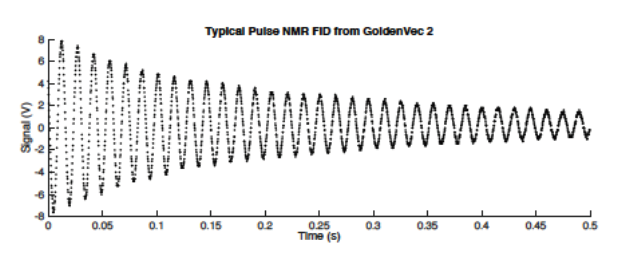
\includegraphics{FID.png}}
	\caption{{\bf A PNMR signal taken with gold coated test cell.}}
	\label{FID}
\end{figure}

Once the optimal settings were found, multiple spindowns were taken. Each spindown was a series of PNMR measurements set apart with fixed time interval. Multiple values of intervals were used for different spindown measurements, each of the intervals was typically repeated at least twice. Fig.~\ref{3spindowns} shows 3 spindowns for the test cell GoldenVec1 which had a horizontal metal tube and similar configuration to that of a convection style cell. The time interval used for the 3 spindowns were 20 min, 30 min and 60 min, respectively. Using the additional relaxation rate due to taking PNMR once every hour as the base rate $\Gamma_{PNMR}$, the measured relaxation rate for taking n PNMR every hour can be related to the true lifetime (without relaxation from PNMR) by:

\begin{equation}
\frac{1}{T_{measured}} = \frac{1}{T_{trure}} + n\cdot \Gamma_{PNMR}
\end{equation}
in the relation of $\frac{1}{T_{measured}}$ versus n, $\frac{1}{T_{trure}}$ is the intercept, and the $\Gamma_{PNMR}$ is the slope.

\begin{figure}[t!]
	\centering
	\resizebox{0.91\textwidth}{!}{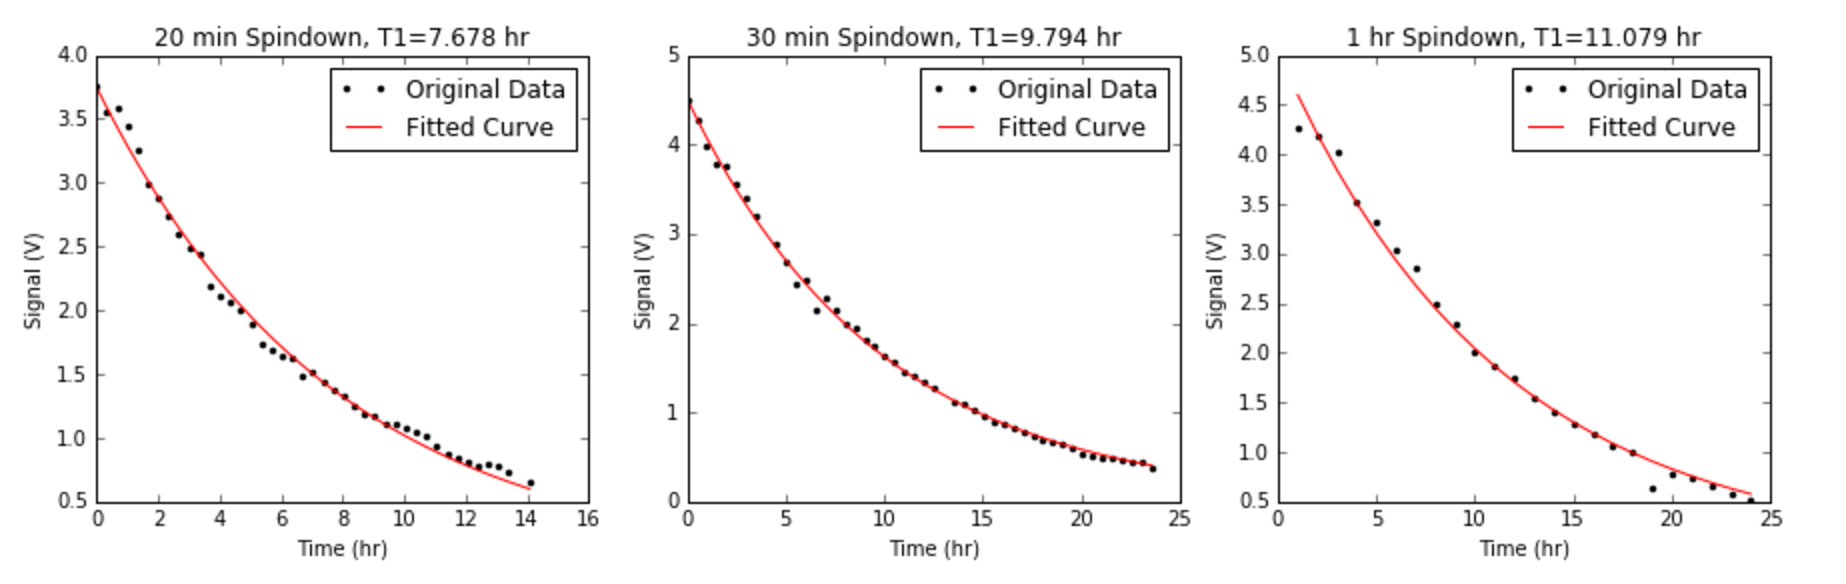
\includegraphics{3spindowns.png}}
	\caption{{3 spindowns of the cell GoldenVec1 each with a different sampling rate.}}
	\label{3spindowns}
\end{figure}

\begin{figure}[t!]
	\centering
	\resizebox{0.91\textwidth}{!}{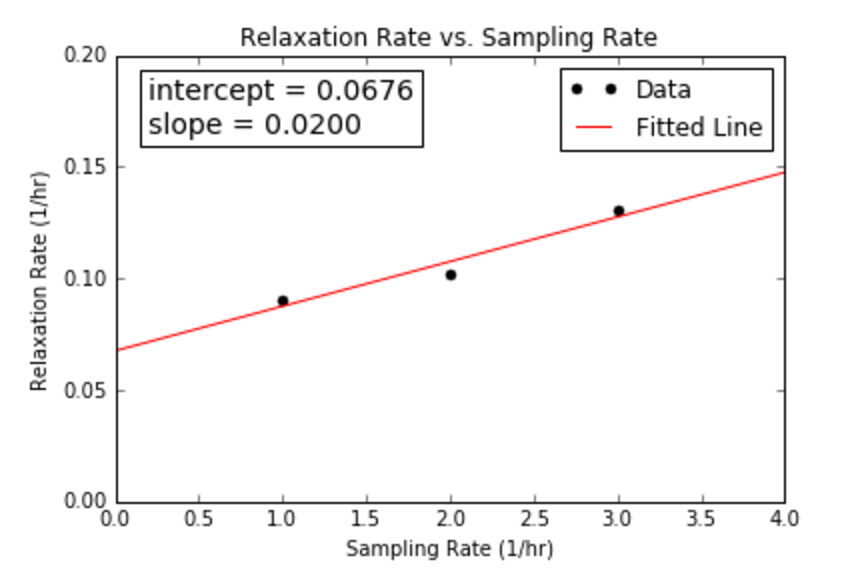
\includegraphics{corrected_T1.png}}
	\caption{{A linear fit to extract lifetime corrected for relaxation due to PNMR losses.}}
	\label{corrected_T1}
\end{figure}

Fig.~\ref{corrected_T1} shows the linear fit between the sampling rates (n) as x and the inverse of measured lifetimes as y. The intercept is $0.0676\,hr^{-1}$, thus the true lifetime without any loss due to taking PNMR measurements is $1/0.0676=14.8\,hr$. The slope is $0.02\,hr^{-1}$, which means the relaxation rate due to taking one PNMR per hour is $1/50\,hr^{-1}$. The percentage loss of polarization due to a single PNMR measurement can be calculated as:

\begin{equation}
1-e^{-t\cdot \Gamma_{PNMR}} = 1-e^{-1\times \frac{1}{50}} =0.0198=2\%
\end{equation}

\section{Relaxation Measurement Results and Discussion}

\begin{figure}[t!]
	\centering
	\resizebox{0.91\textwidth}{!}{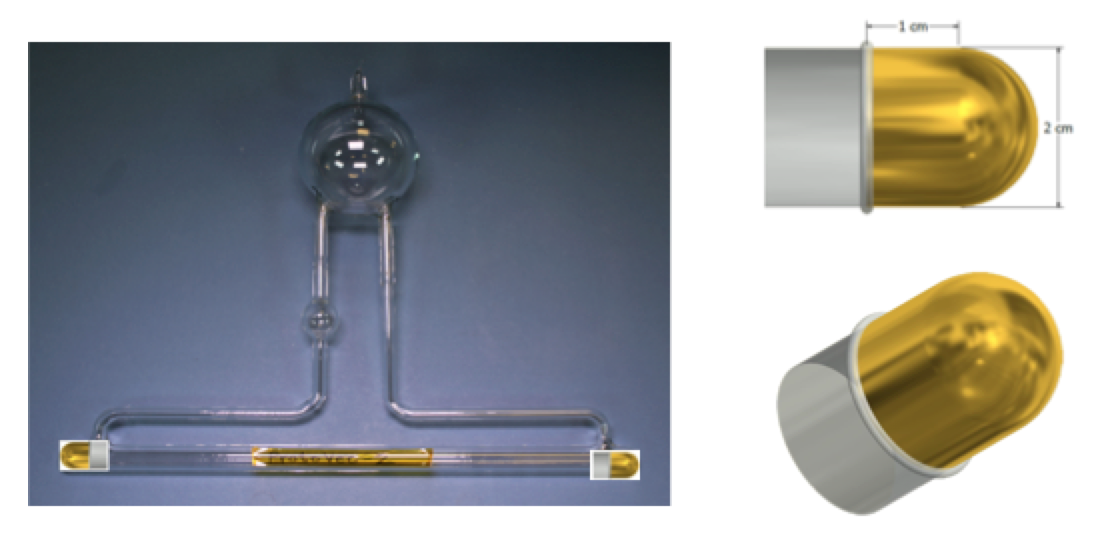
\includegraphics{metal_end_windows.png}}
	\caption{{A diagram of target cell with metal end windows. }}
	\label{metal_end_windows}
\end{figure}

The end goal of this series of studies is to replace the traditional glass windows on target chamber with metal end windows as Fig.~\ref{metal_end_windows} shows. Although no metal end windows have been produced yet, 19 test cells with various configurations and compositions were studied to explore the feasibility of incorporating metallic components into glass cells. We have gone through different stages of studies, from each we made new discoveries and stepped closer to the end goal. At this point, we have demonstrated that gold coated OFHC copper is strong enough to survive the high gas pressure of electron scattering experiments, only brings a relatively small amount of relaxation rates to a convection style target cell made with GE180 under SEOP conditions. The following discussion will be separated into different stages that each revealed parts of the mystery and generally follow chronological order (except cells made with titanium will be covered at the end). The cell preparation information and results of measurements are listed in Table~\ref{test_cells}.

\begin{table*}\scriptsize
	\captionsetup{font=scriptsize}
	\begin{center}
		\def\arraystretch{0.75}
		\setlength\tabcolsep{2pt}
		\begin{tabular}{|c|c|c|c|c|c|c|}
			\hline
			Cell Name & Fill Type & Geometry & Glass & Metal & Max Lifetime (hr) & Fill Date\\ \hline
			Tyrion & NGP & Sphere & GE180 & Gold on glass & 1.21 & 6/18/09 \\ \hline
			Gold Maiden1 & NGP & Flange & Pyrex & Gold on Copper & 2.14 & 6/18/10 \\ \hline
			Gold Maiden2 & NGP & Flange & Pyrex & Gold on Copper & None & 8/14/10\\ \hline
			Gold Maiden3 & NGP & Flange & Pyrex & Gold on Copper & 6.49 & 11/11/10\\ \hline
			Goldfinger & NGP & Vertical & Pyrex & Gold on Copper & 3.59 & 4/28/13\\ \hline
			Cupid & NGP & Vertical & Pyrex & Bare Copper & 3.13 & 6/15/13\\ \hline
			Goldeneye & NGP & Vertical with Valve & Pyrex & Gold on Copper & 13.94 & 10/2/13\\ \hline
			GoldRush & NGP & Vertical & Pyrex & Gold on Copper & 14.81$^\dagger$  & 11/8/13\\ \hline
			Pyrah & NGP & Vertical & Pyrex & None & 26.52$^\dagger$ & 2/1/14\\ \hline
			GoldenVec & NGP & Horizontal & Pyrex & Gold on Copper & 10.6 & 10/18/14\\ \hline
			TitanVec & NGP & Horizontal & Pyrex & Gold on Titanium & 0.52 & 12/15/14\\ \hline
			GoldenVec2 & Cryogenic & Horizontal & Pyrex & Gold on Copper & 15.6 & 2/14/15\\ \hline
			Titan & NGP & Vertical & Pyrex & Bare Titanium & None & 3/11/15\\ \hline
			GoldenVec180 & Cryogenic & Horizontal & GE180 & Gold on Copper & 4.43 & 6/17/15\\ \hline
			GolderVec360 & Cryogenic & Horizontal & GE180 & Gold on Copper & 3.01 & 7/11/15\\ \hline
			Tweety & Cryogenic & Vertical & Pyrex & Canary Glass & 22.7 & 9/22/15 \\ \hline
			Sylvester & Cryogenic & Horizontal & GE180 & Canary Glass & 6.39 & 11/20/15\\ \hline
			Kappa1 & Cryogenic & Sphere & GE180 & None & 72.17 & 2/6/16\\ \hline
			Goldfinger180 & Cryogenic & Vertical & GE180 & Gold on Copper & 12.4 $^\dagger$ & 5/19/16\\ \hline
		\end{tabular}
		\caption
		{Shown are the fill information, design and maximum measured lifetime of the test cells. Fill type is the method used to clean the gas. $^\dagger$ indicates the maximum lifetime was obtained at an elevated position. Although canary glass is not metal, it is listed in the column of metal for Tweety and Sylvester for the sake of keeping the structure of the table simple.}
		\label{test_cells}
	\end{center}
\end{table*}

\subsection{Gold Coated Spherical Cell}

Our very first attempt at incorporating metal was a spherical GE180 cell with gold coated on the interior surface. The measured lifetime was only 1.21 hr, which was attributed to impurities in the cell. Although this attempt was made before I joined the group as were the spool pieces that will be mentioned below, they are still included for the sake of completeness of this study. 

\subsection{Gold Coated Spool Pieces}

The first cell with a gold coated (by Epner) OFHC copper tube was named as "Gold Maiden" and made in 2010. Fig.~\ref{spool_piece} is a picture of the cell which was referred to as the "spool piece". The bottom end of the cell was capped off, while the other end was attached to a glass flange. The flange was then connected to the transfer tube of the cell. The seal was made with o-rings. 

\begin{figure}[t!]
	\centering
	\resizebox{0.15\textwidth}{!}{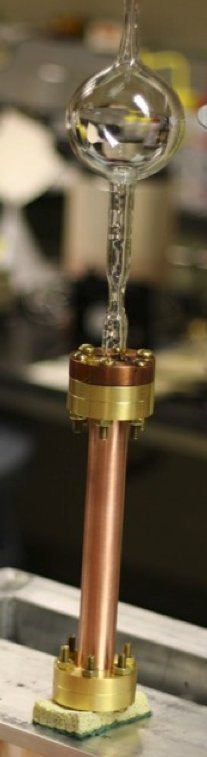
\includegraphics{spool_piece.png}}
	\caption{{A picture of Gold Maiden, generally referred to as the "spool piece". }}
	\label{spool_piece}
\end{figure}

The tests of Gold Maiden was divided into three stages. Initially it had a lifetime of 2.14 hr before discoloration of Rb was observed. The discoloration is typically a sign of Rb reacting away with air, which indicated either a leak or significant amount of outgassing from the o-rings. To separate Rb from possible outgassing, the pumping chamber was pulled off via glassblowing. Measurements of the separated pumping chamber showed a lifetime of 109.2 hr after correcting for AFP losses. The rest of the cell which contained the transfer tube and the metal tube was measured again with PNMR, and a lifetime of 6.49 hr was recorded. The spool piece encouraged further investigation into gold coated OFHC copper that could be attached to glass without o-rings.

\subsection{Vertical Cells}

Since o-rings were the primary suspects of the short lifetime for the spool piece, a method to seal copper directly to the glass was highly desirable. We started using the Houskeeper seal, and five cells were made at this stage: Goldfinger, Cupid, Goldrush, Goldeneye and Pyrah. All 5 cells were designed to have the same dimensions. Fig.~\ref{goldfinger} shows the design drawing and a picture of the cell Goldfinger. Goldrush was of the same design. The only difference for Cupid was that the OFHC copper was not coated. Pyrah was a pure Pyrex control cell. 

\begin{figure}[t!]
	\centering
	\resizebox{0.65\textwidth}{!}{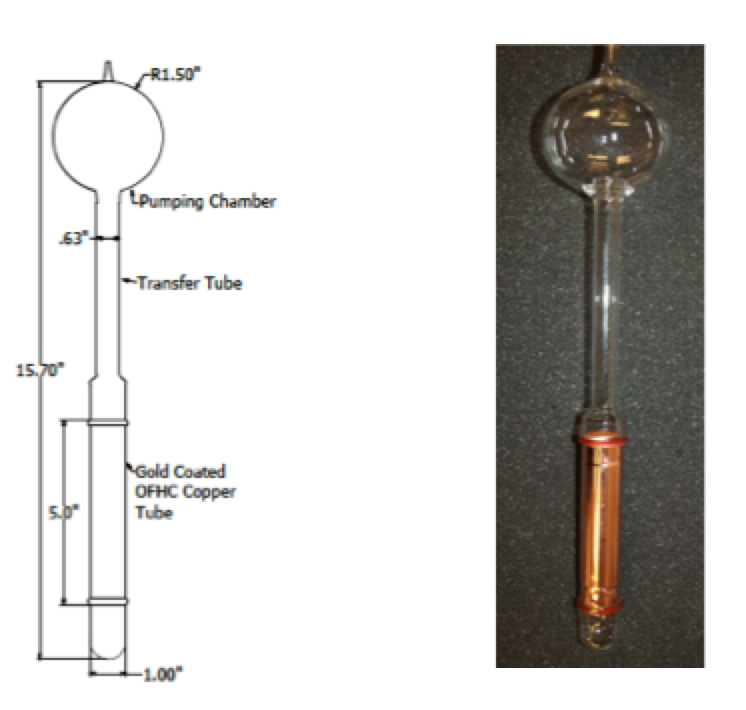
\includegraphics{goldfinger.png}}
	\caption{{Design and picture of Goldfinger. }}
	\label{goldfinger}
\end{figure}

Goldfinger had a maximum lifetime of 3.59 hr at the beginning of the test. However, subsequent tests showed a somewhat obvious degradation. Towards the end of testing Goldfinger, the lifetime was at a minimum of 2.36 hr. Cupid had a similar maximum lifetime of 3.13 hr initially. A even more significant degradation of lifetime was observed with Cupid. The last measurement we were able to perform displayed only 0.27 hr. It is worth noting a leak on Goldfinger was discovered during the filling process. Although the leak was fixed with Celvaseal Leak Sealant, either the sealant or the leak itself might have contributed to the short lifetime of Goldfinger and its degradation. Rb is also known to form amalgam with copper, which could be the reason for the observed behavior of Cupid. Fig.~\ref{T1_degradation} displays the lifetime degradation during our tests.

\begin{figure}[t!]
	\centering
	\resizebox{0.91\textwidth}{!}{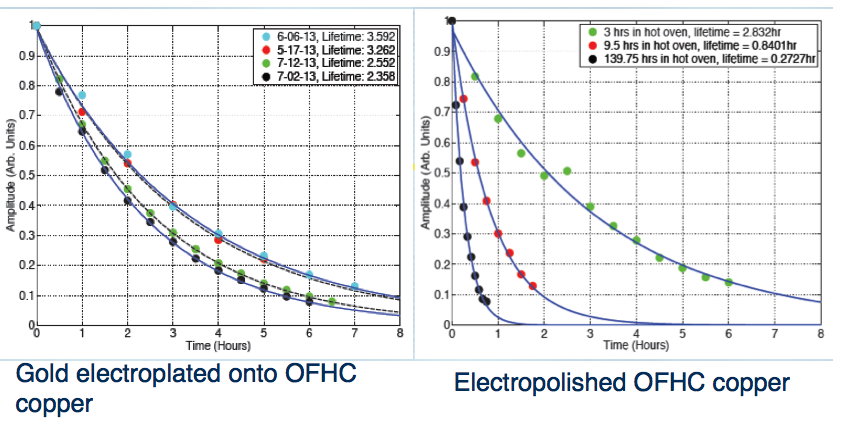
\includegraphics{T1_degradation.png}}
	\caption{{The observed degradation of lifetime for Goldfinger (left) and Cupid (right). Shown in each of the two plots were several spindowns at different stage during the tests. The initial amplitude of the spindowns were scaled to 1 for better comparison of lifetime.}}
	\label{T1_degradation}
\end{figure}

During the tests of Goldfinger and Cupid, it was suspected that Rb reacted with metal surfaces and produced detrimental effects to lifetime. A gold coated OFHC cell with valve was designed and produced to isolate Rb vapor from the metal tube, as shown in Fig.~\ref{goldeneye}. GoldenEye was only polarized after the valve was closed, thus Rb vapor should never reach the metal tube. Spindown measurements were taken at room temperature both with the valve closed and open. The lifetime was measured to be 13.94 hr with the valve closed, and it was only 4.09 hr with the valve open. The large difference of lifetime indicated the part of the cell below the valve introduced very significant relaxation rate. It is also worth noting the inclusion of the valve increased the total length of the cell substantially, which exposed the bottom part of the cell to high field inhomogeneities that could lead to high relaxation rate.

\begin{figure}[t!]
	\centering
	\resizebox{0.15\textwidth}{!}{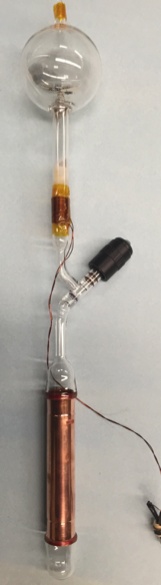
\includegraphics{goldeneye.png}}
	\caption{{A picture of GoldenEye, the only test cell made with a valve.}}
	\label{goldeneye}
\end{figure}

Due to the leak found in Goldfinger, it was necessary to produce another test cell with the same design, which was named as ``Goldrush". Fig.~\ref{goldrush} display four spindowns taken before elevating the cell. All four measurements have similar results with the maximum lifetime being 12.1 hr. This was the first metal cell we produced that had more than 10 hr lifetime. 

\begin{figure}[t!]
	\centering
	\resizebox{0.91\textwidth}{!}{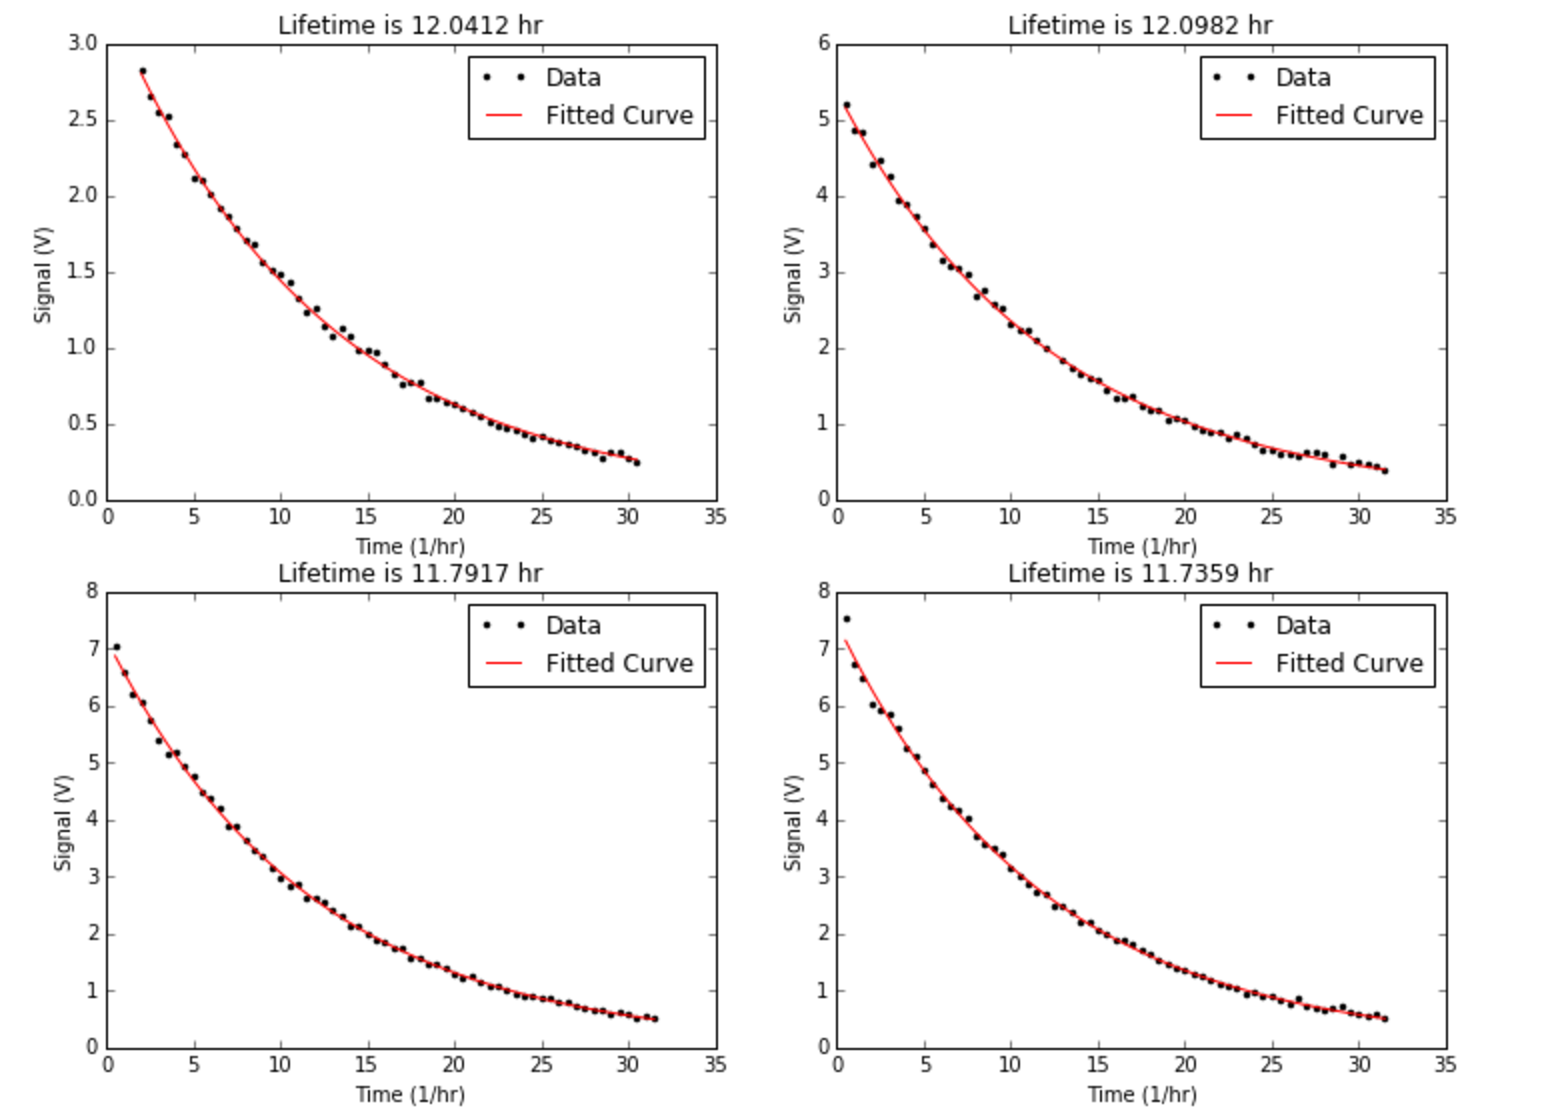
\includegraphics{goldrush.png}}
	\caption{{Four spindowns of Goldrush before elevating the cell. All four measurements display similar lifetime with no obvious sign of degradation.}}
	\label{goldrush}
\end{figure}

A calculation of the magnetic field inhomogeneities was also done around the time. As seen in Fig.~\ref{goldrush_inhomogeneities}, the relaxation time due to inhomogeneities at the center of the pumping chamber was about 300-700 hr. However, the bottom of cell was exposed to surprisingly large inhomogeneities which would result in a relaxation time of 1-5 hr. This provided incentive for measurements of lifetime while raising the cell to more homogeneous region. Due to spatial constraints, the cell was only lifted by 10 cm, which led to an increase in lifetime to 14.81 hr, the longest lifetime we had measured at the time with metal cells.

\begin{figure}[t!]
	\centering
	\resizebox{0.91\textwidth}{!}{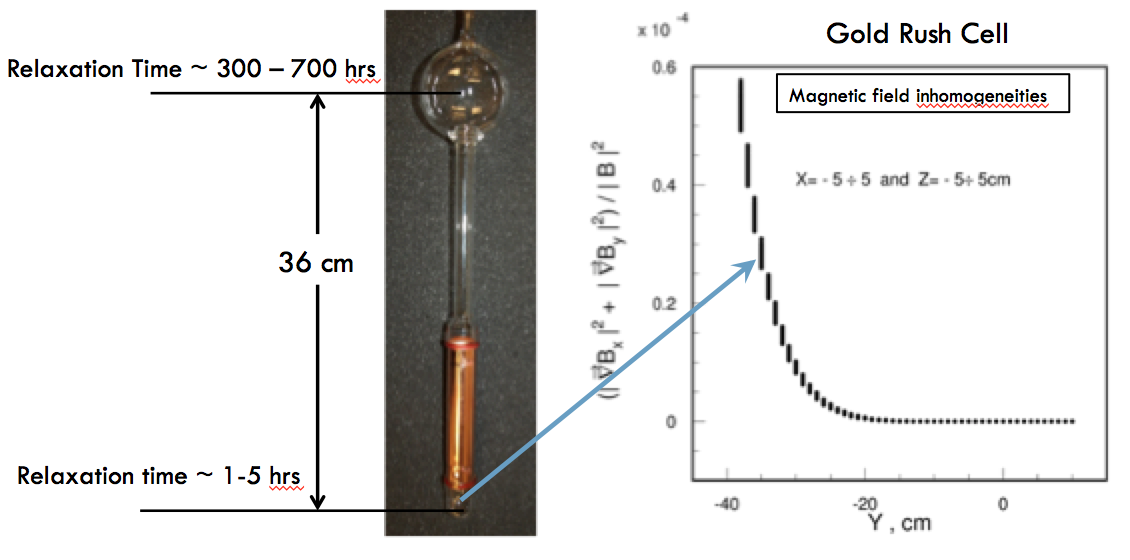
\includegraphics{goldrush_inhomogeneities.png}}
	\caption{{Shown on the right is the inhomogeneities vs. vertical distance from the center of the field. Shown on the left is the cell Goldrush with relaxation time due to field inhomogeneities as displayed on the right.}}
	\label{goldrush_inhomogeneities}
\end{figure}

To understand the additional relaxation rates introduced by metal surfaces, a control cell, Pyrah, was made with pure Pyrex was produced. The control cell had a lifetime of 19.71 hr before elevation, and 26.52 hr after being lifted by 10 cm. Since Pyrah had the same dimensions as Goldrush, a direct comparison suggested the additional relaxation rate due to the metal tube was around $1/25\,hr$.

\subsection{Horizontal Cells}

The increase of lifetime after elevating Goldrush and Pyrah motivated us to make more compact cell designs. This resulted in a design very similar to that of a convection style cell with the metal tube placed horizontally. The overall vertical length was shortened from 15.75'' to about 10''. The dimensions of this style of cells can be seen in Fig.~\ref{goldenvec}.

\begin{figure}[t!]
	\centering
	\resizebox{0.6\textwidth}{!}{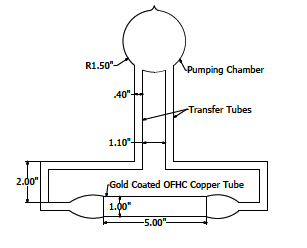
\includegraphics{goldenvec.png}}
	\caption{{Design of the horizontal cell GoldenVec.}}
	\label{goldenvec}
\end{figure}

The first horizontal cell was GoldenVec. It had a lifetime of 10.6 hr, which was shorter than we had hoped for. Up to this point, all test cells were filled using the noble gas purifier in our lab. A convection cell filled at the time that used the cryogenic trap to condense the impurities in the gas turned out to have much greater lifetime compared to the previous convection cell of the same design but used the noble gas purifier. In light of this, GoldenVec2 was created with the same design as that of GoldenVec and the cryogenic trap. GoldenVec2's lifetime was measured to be 15.6 hr, the longest lifetime of metal cells we have obtained to date. All test cells from then on were filled using the same cryogenic trap.

\subsection{GE180 Cells}

It was widely acknowledged that the impermeable aluminosilicate glass GE180 had less associated wall relaxation rates than that of the borosilicate glass Pyrex. Since GoldenVec2 and Goldrush had demonstrated good enough lifetime, it was time we started exploring GE180 cells with metal tubes. Two GE180 test cells, GoldenVec180 and GoldenVec360, were made with the design as seen in Fig.~\ref{goldenvec}. Because of the difficulty in bonding GE180 to OFHC copper, Corning 7052 was used as the transition glass. The measured lifetime of GoldenVec180 and GoldenVec360 were 4.43 hr and 3.01 hr, respectively. Since GE180 glass normally provide longer relaxation time, we made additional cells to test different hypothetical interpretation of the short lifetime.

The first suspect occurred to us was the transition glass Corning 7052, since it had never been tested in our group. As we had experience with an alternative transition glass, canary glass (uranium glass), we built two test cells with 5'' long by 1'' OD  tubes of the canary glass in place of copper tubes. The first was a replicate of the vertical cell Goldfinger and named as Tweety. The second was a replicate of the horizontal cell GoldenVec and named as Sylvester.

Tweety had a lifetime of 22.7 hr, which was quite close to the lifetime of the control cell Pyrah, 26.52 hr. A shorter lifetime was expected as uranium is paramagnetic, however, the result of Tweety proved the expectation was incorrect and canary glass could in fact be used to build target cell.

Results of Sylvester was also unexpected as the lifetime was only 6.39 hr even in the absence of metal. This lifetime was shorter than that of GoldenVec and GoldenVec2. At this point, we narrowed down the causes of such short lifetime to the last two:
1. The melt of the GE180 glass had too much impurities.
2. Insufficient annealing resulted in more remaining micro-fissures in the glass.

The first possibility is easy to understand and could be easily tested with a simple spherical cell built from the same melt of GE180. Kappa1 was produced for this exact purpose. Hybrid Mixture of Rb and K was used instead of Rb because Kappa1 was also intended for future measurements of the physical quantity $\kappa_0$ which require hybrid mixtures. Kappa1 was found to have a lifetime of 72 hr, so the cause of high relaxation in previous GE180 cells was not the melt itself.

As mentioned in previous sections, to keep the glass-metal seals intact, all glass parts not directly attached to metal tubes were placed in a oven for annealing. Larger amount of micro-fissures could still exist in the glass directly attached to metal. This could potentially lead to the short lifetime we observed with the GE180 cells up to this point. To test the hypothesis, Goldfinger180 was built following the design of Goldfinger. However, the glass directly attached to the metal tube that did not go into the oven was intentionally made shorter by our glassblower. During the fill process, a leak at the Houskeeper seal had to be fixed with two coats of an epoxy sealant Stycast 1266. The lifetime was measured to be 10.4 hr before elevation, and 12.4 hr after elevating in the same manner as Goldrush and Pyrah. The result both demonstrated the feasibility of using gold coated OFHC copper with GE180 and further confirmed the significance of glass annealing.

\subsection{Titanium Tubes}

Although gold coated OFHC copper was the main focus of the study due to the ease of manufacturing, titanium was also investigated for its stronger tensile strength and lower atomic number. However, the results of the two titanium cells were not satisfactory. A test cell with bare titanium tube, Titan, had lifetime too short to be measured. The other cell TitanVec with gold coated titanium tube had lifetime of only 0.52 hr. Because of the difficulty in coating gold onto titanium surface, parts of gold coating peeled off the surface during the cleaning process with our ultrasonic cleaner. $^{3}$He was exposed to part of the titanium surface underneath, which could be the reason for the bad relaxation properties. As a result, titanium was not investigated further.





